\documentclass[10pt,xcolor=pdflatex,hyperref={unicode},aspectratio=169]{beamer}
\usepackage{newcent}
\usepackage{animate}
\usepackage[utf8]{inputenc}
\usepackage[czech]{babel}
%\usepackage[T1]{fontenc}
\usepackage{hyperref}
\usepackage{fancyvrb}
\usetheme{FIT}

\newcommand{\btVFill}{\vskip0pt plus 1filll}

%%%%%%%%%%%%%%%%%%%%%%%%%%%%%%%%%%%%%%%%%%%%%%%%%%%%%%%%%%%%%%%%%%
\title[Diplomová práce]{Simulace kapalin na GPU }

\author[]{Bc. Igor Frank}

\institute[]{Brno University of Technology, Faculty of Information Technology\\
Bo\v{z}et\v{e}chova 1/2. 612 66 Brno - Kr\'alovo Pole\\
xfrank12@fit.vutbr.cz}

%\institute[]{Fakulta informačních technologií
%Vysokého učení technického v Brně\\
%Bo\v{z}et\v{e}chova 1/2. 612 66 Brno - Kr\'alovo Pole\\
%login@fit.vutbr.cz}

% České logo - Czech logo
% beamerouterthemeFIT.sty řádek 9: fitlogo1_cz

\date{\today}
%\date{\today}
%\date{} % bez data / without date

%%%%%%%%%%%%%%%%%%%%%%%%%%%%%%%%%%%%%%%%%%%%%%%%%%%%%%%%%%%%%%%%%%

\begin{document}

\frame[plain]{\titlepage}

\begin{frame}\frametitle{Zadání}

    \begin{center}
        Simulace kapalin na GPU
        
        \textit{Fluid Simulation Using GPU}
        \bigbreak
        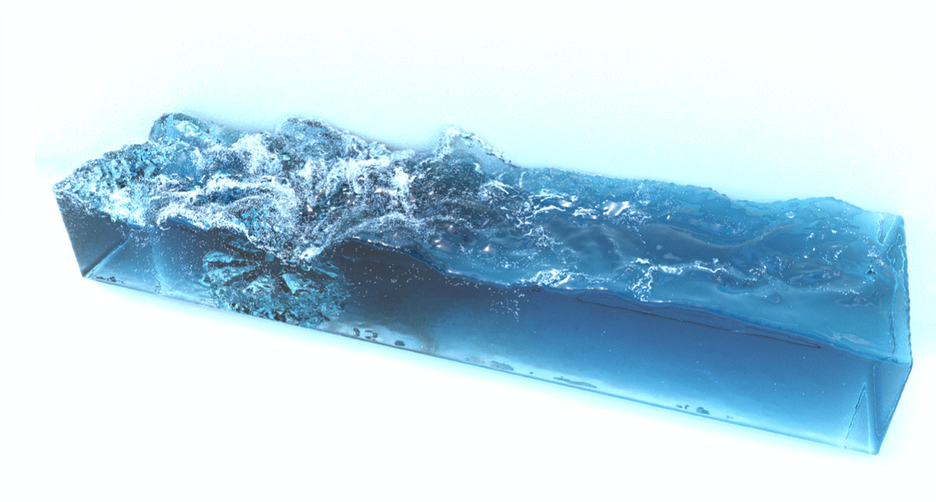
\includegraphics[scale=0.3]{img/fluid.png}%
    \end{center}

\end{frame}

%--------------------------

\begin{frame}\frametitle{Cíl}
    \begin{columns}
        \hspace{.4cm}
        \begin{column}{0.5\textwidth}
            \textbf{Studium}
            \begin{itemize}
                \item Vulkan API
                \item Metody simulace kapalin
            \end{itemize}
        \end{column}
        \begin{column}{0.5\textwidth}
            
\includegraphics[scale=0.2]{img/Vulkan.png}
        \end{column}
    \end{columns}
    
    \bigbreak
    \bigbreak
    
    \textbf{Implementace článku} \\
    \textit{Evaporation and condensation of SPH-based fluids} \footnote{Hochstetter, H. a Kolb, A. Evaporation and condensation of SPH-based fluids. In:. červenec 2017, s. 1–9. DOI: 10.1145/3099564.3099580. ISBN 978-1-4503-5091-4}
    \begin{itemize}
        \item Metoda pro simulování vypařování a kondenzace
        \item Různé přístupy k simulaci a jejich propojení
    \end{itemize}

\end{frame}

%--------------------------

\begin{frame}{Základní vlastnosti}
    \begin{columns}
        \hspace{.4cm}
        \begin{column}{0.5\textwidth}
            Akcelerace výpočtů za pomocí GPGPU
            \bigbreak
            Simulace dvou skupenství kapalin
            \begin{itemize}
                \item Částicová simulace (Smoothed~particle~hydrodynamics)
                \item Mřížková simulace
                \item Propojení pomocí vypařování
            \end{itemize}
            \bigbreak
            Vizualizace průběhu simulace
        \end{column}
        \begin{column}{0.5\textwidth}
            \begin{center}
                \animategraphics[loop, autoplay, width=0.7\linewidth]{30}{img/video6/Untitled-Prez_}{000000}{000290}
            \end{center}
        \end{column}
    \end{columns}
    
\end{frame}

%--------------------------

%--------------------------

\begin{frame}{SPH simulace}
        \begin{columns}
            \hspace{.4cm}
            \begin{column}{0.5\textwidth}
            \begin{center}
                \animategraphics[loop, autoplay, width=0.7\linewidth]{30}{img/video6/Untitled-Prez_}{000000}{000290}
            \end{center}
        \end{column}
        \begin{column}{0.5\textwidth}
            \begin{itemize}
                \item Částicová metoda WCSPH
                \item Využití mřížkové vyhledávací struktury
            \end{itemize}
        \end{column}
    \end{columns}

    
\end{frame}

%--------------------------

\begin{frame}{SPH simulace}
        \begin{columns}
            \begin{column}{0.5\textwidth}
            Konfigurace simulace
            \begin{itemize}
                \item Délka kroku
                \item Hustota
                \item Viskozita
                \item ...
            \end{itemize}
        \end{column}
            \begin{column}{0.5\textwidth}
            \begin{center}
                \animategraphics[loop, autoplay, width=0.7\linewidth]{30}{img/video6/Untitled-Prez_}{000000}{000290}
            \end{center}
        \end{column}
    \end{columns}

    
\end{frame}
%--------------------------

\begin{frame}{Simulace vypařování}
        \begin{columns}
            \hspace{.4cm}
            \begin{column}{0.5\textwidth}
            \begin{center}
                \animategraphics[loop, autoplay, width=0.7\linewidth]{30}{img/video6/Untitled-Prez_}{000000}{000290}
            \end{center}
        \end{column}
        \begin{column}{0.5\textwidth}
            Přenos hmoty
            
            Přenos tepla
            \bigbreak
            Závisí na:
            \begin{itemize}
                \item Teplotě okolí
                \item Teplotě kapaliny
                \item Proudění vzduchu
            \end{itemize}
        \end{column}
    \end{columns}
    
\end{frame}

%--------------------------

\begin{frame}{Vykreslování}

    \begin{columns}
        \hspace{.4cm}
        \begin{column}{0.5\textwidth}
            \begin{itemize}
                \item Instancované vykreslování
                \bigbreak
                \item Marching-cubes
                \bigbreak
                \item Vizualizace hustoty kapaliny
            \end{itemize}
        \end{column}
            \begin{column}{0.5\textwidth}
            \begin{center}
                \animategraphics[loop, autoplay, width=0.7\linewidth]{30}{img/video6/Untitled-Prez_}{000000}{000290}
            \end{center}
        \end{column}
    \end{columns}
    
    \begin{columns}
        \hspace{.4cm}
        \begin{column}{0.5\textwidth}
            \begin{center}
                \animategraphics[loop, autoplay, width=0.7\linewidth]{30}{img/video6/Untitled-Prez_}{000000}{000290}
            \end{center}
        \end{column}
        \begin{column}{0.5\textwidth}
            \begin{center}
                \animategraphics[loop, autoplay, width=0.7\linewidth]{30}{img/video6/Untitled-Prez_}{000000}{000290}
            \end{center}
        \end{column}
    \end{columns}
    
\end{frame}

%--------------------------

\begin{frame}{Rozšířené funkce aplikace}

        \begin{columns}
            \hspace{.4cm}
            \begin{column}{0.5\textwidth}
            \begin{itemize}
                \item Ovládání simulace
                \item Nahrávání videa
                \item Pořizování snímků
                \item Uložení stavu simulace
                \item Nastavení světla, barvy kapaliny
            \end{itemize}
        \end{column}
            \begin{column}{0.5\textwidth}
            \begin{center}
                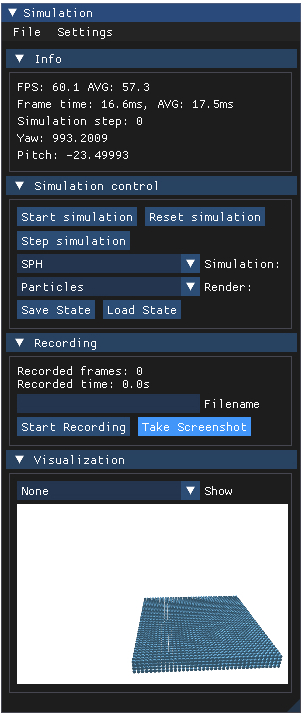
\includegraphics[scale=1]{img/Main.jpg}
            \end{center}
        \end{column}
    \end{columns}
    
\end{frame}

%--------------------------

\begin{frame}{Časová náročnost}
    \bigskip
    \bigskip
    \bigskip
    \begin{table}[]
        \begin{tabular}{l|c|c|c|c}
            Scénář            & Počet částic & Počet buněk & SPH simulace & Grid simulace \\ \hline
            Akvárium & 27000        & -                                    & 3,8 ms       & -                                     \\
            Kolize            & 55800        & -                                    & 6,0 ms       & -                                     \\
            Vypařování        & 5476         & $20^3$                                   & 2,6 ms       & 16,8 ms                              
        \end{tabular}
    \end{table}
    \btVFill
    \begin{columns}[]
            \hspace{1.5cm}
            \begin{column}{0.49\textwidth}
                Nastavení
                \begin{itemize}
                    \item $\Delta t = 0.001s$
                    \item $k = 100J$
                \end{itemize}
                \vspace{\baselineskip}
            \end{column}
                \begin{column}{0.49\textwidth}
                Systém
            \begin{itemize}
                \item AMD Ryzen 5 5600X
                \item Nvidia RTX 3070 (8GB VRAM)
                \item 16 GB RAM
            \end{itemize}
            \end{column}
    \end{columns}
    \bigskip
    \bigskip
\end{frame}

%--------------------------

\bluepage{Děkuji za pozornost !}

%--------------------------

\begin{frame}\frametitle{Výsledek}
    \animategraphics[loop, autoplay, width=0.5\linewidth]{30}{img/video6/Untitled-Prez_}{000000}{002477}
\end{frame}

\end{document}
